\subsection{Punt in veelhoek}
\label{sub:algo-pt-in-poly}
Eén van de voorwaarden waaraan een oplossing moet voldoen is dat alle punten \textbf{in} de veelhoek liggen.Het is dus noodzakelijk om een algoritme te hebben dat bepaalt of een punt zich al dan niet in de convexe veelhoek bevind.
\subsubsection{Idee}
Trekken we een lijn vanuit het punt ``naar boven'', dan kunnen we 3 gevallen onderscheiden:
\begin{itemize}
\item We snijden de veelhoek niet ($P_{1}$): \\
		We weten dat we ons niet binnen de veelhoek bevonden.
\item We snijden de veelhoek juist 1 keer ($P_{2}$):\\
		Nu zijn we zeker in de veelhoek. 
\item We snijden de veelhoek juist\footnote{Merk op dat indien we de veelhoek meer dan 2 keer snijden, we kunnen aantonen dat de veelhoek niet convex is.} 2 keer ($P_{3}$):\\
		We liggen onder en dus ook buiten de veelhoek.
\end{itemize}

\begin{center}
\begin{figure}[H]
\centering
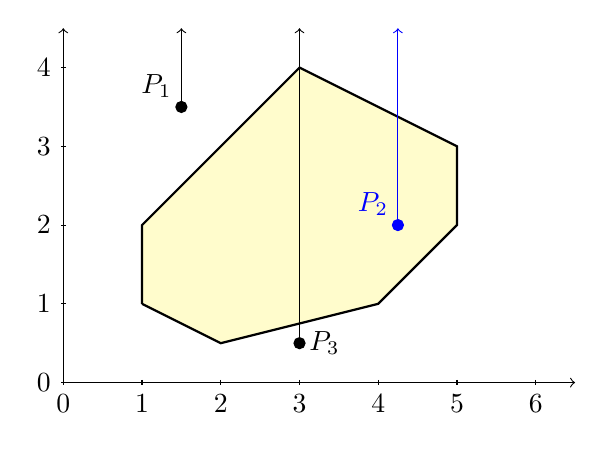
\begin{tikzpicture}
\draw[->] (0,0) -- (6.5,0);
\draw[->] (0,0) -- (0,4.5);

\foreach \x in {0,1,2,3,4,5,6}
    \draw (\x cm,1pt) -- (\x cm,-1pt) node[anchor=north] {\x};
\foreach \y in {0,1,2,3,4}
    \draw (1pt,\y cm) -- (-1pt,\y cm) node[anchor=east] {\y};

\draw[thick,fill=yellow, fill opacity=0.2] 
      (1,1) -- (1,2) -- 
	  (3,4) -- (5,3) -- 
	  (5,2) -- (4,1) -- 
	  (2,0.5) -- (1,1);
	  
	  
\coordinate (out1)    at (1.5,3.5);
\coordinate (out1top) at (1.5,4.5);
\filldraw[black] (out1) circle (2pt) node[anchor=south east] {$P_{1}$};

\coordinate (out2)    at (4.25,2);
\coordinate (out2top) at (4.25,4.5);
\filldraw[blue] (out2) circle (2pt) node[anchor=south east] {$P_{2}$};

\coordinate (out3)    at (3,0.5);
\coordinate (out3top) at (3,4.5);
\filldraw[black] (out3) circle (2pt) node[anchor=west] {$P_{3}$};


\draw[->] (out1) -- (out1top);
\draw[->,blue] (out2) -- (out2top);
\draw[->] (out3) -- (out3top);
\end{tikzpicture}
\caption{Punten binnen en buiten de figuur \texttt{soos.poly} met snijpunten.}
\end{figure}
\end{center}
We moeten dus nagaan dat een lijn ``naar boven'' vanuit het punt de veelhoek
juist één keer snijd.


\subsubsection{Algoritme}
Om te tellen hoe vaak we de veelhoek snijden, gaan we als volgt te werk:
Bij het inlezen van de veelhoek stellen we vergelijkingen op van de zijden van de 
veelhoek. Deze zijn van de vorm $y=a \cdot x+b$. Met $a = \infty$ als de rechte evenwijdig is met de $y$-as. 



	\begin{algorithm}[H]
	 	\caption{Bepalen of een punt in een veelhoek ligt}
		\begin{algorithmic}
		\Require zijden, een lijst van de zijden van een convexe veelhoek.
		%\Ensure T is gebalanceerd
		\Function{inPolygon}{$P_x$,$P_y$}
		\State count $\gets$ 0
		
		\For{\textbf{each} z $\in$ zijden} 
		\State $(x_1,y_1)$ $\gets$ $1^{ste}$ gedefinieerde punt van z
		\State $(x_2,y_2)$ $\gets$ $2^{de}$ gedefinieerde punt van z
		\If{z.$a = \infty$} 	\Comment Als z $\parallel$ $y$-as 
			\If{$P_y \in  \left \lbrack y_1,y_2\right\lbrack$}
			\State \Return \texttt{true} \Comment{Op lijn}
			\ElsIf{$y_1 > P_y$}
				\State count $\gets$ count$+1$
			\EndIf
		\Else	\Comment z $\not \parallel$ $y$-as
			\State $y_{inter}  \gets$ z.$a\cdot P_x +$z.$b$
			\If{$P_x \in  \left \lbrack x_1,x_2\right\lbrack$}
			
			\If{ $y_{inter} = P_y$ } 
				\State \Return \texttt{true} \Comment{Op lijn}
			\ElsIf{ $y_{inter} > P_y $} 
				\State count $\gets$ count$+1$
			\EndIf
				
			\EndIf
		\EndIf	

		\EndFor		

		\Return count == 1 ? \texttt{true} : \texttt{false}
		\EndFunction
		\end{algorithmic}
		\label{alg:inPolygon}
	\end{algorithm}		

Waarbij z$.a$ en z$.b$ de cooificienten zijn van de vergelijking $y=ax+b$ die de zijde 
voorstelt 

\subsubsection{Complexiteit}
Kijken we naar algoritme \ref{alg:inPolygon} dan is het duidelijk dat de complexiteit $O(z)$ is met $z$ het aantal zijden.

% subsection  (end)

\subsubsection{Implementatie}
Deze methode is geimplementeerd in \texttt{polygon.c} als \texttt{polygon\_contains()}. 
We wijzen nog even op enkele details:
\begin{itemize}
\item We gebruiken $(P_x-x_1)\cdot(P_x-x_2)\leq0$ om te bepalen of een waarde al dan niet 
		tussen 2 waarden ligt. We doen dit zo omdat we niet weten hoe $x_1$ en $x_2$ 
		zich onderling verhouden.
\item Om het herberekenen van $a$ en $b$ te vermijden, berekenen we deze eenmalig bij het inlezen van de veelhoek.

\end{itemize}

% subsection  (end)

 
